%%%%%%%%%%%%%%%%%%%%%%%%%%%%%%%%%%%%%%%%%%%%%%%%%%%%%
%%% Task 4 %%%%%%%%%%%%%%%%%%%%%%%%%%%%%%%%%%%%%%%%%%
%%%%%%%%%%%%%%%%%%%%%%%%%%%%%%%%%%%%%%%%%%%%%%%%%%%%%
\task{B6C converter at a motor load}

\taskGerman{B6C Umrichter bei Motorlast}

An industrial DC motor is used in a rolling mill drive, powered through a B6C six-pulse controlled rectifier, 
shown in \autoref{fig:B6C_topology_WithMotor}, from a three-phase $\SI{480}{\volt}$, $\SI{50}{Hz}$ grid. The motor has a rated terminal voltage of $\SI{400}{\volt}$
and draws $\SI{50}{\ampere}$. A large smoothing inductor ($L \to \infty$) ensures constant output current. 
The converter is utilized to operate in motoring mode by adjusting the firing angle $\alpha$.

\begin{germanblock}
    Ein industrieller Gleichstrommotor wird in einem Walzwerksantrieb verwendet, der über einen B6C-Sechs-Puls-Gleichrichter
(siehe \autoref{fig:B6C_topology_WithMotor}) aus einem dreiphasigen $\SI{480}{\volt}$, $\SI{50}{Hz}$ gespeist wird. Der Motor hat eine Nennankerspannung
von $\SI{400}{\volt}$ und zieht $\SI{50}{\ampere}$. Eine große Glättungsinduktivität ($L \to \infty$) sorgt für einen konstanten Ausgangsstrom.
 Der Umrichter wird durch Einstellen des Zündwinkels $\alpha$ im Motorbetrieb betrieben.
\end{germanblock}
%%%%%%%%%%%%%%%%%%%%%%%%%%%%%%%%%%%%%%%%%%%%%%%%%%%%%%%%%%%%%%%%%%%%%%%
 % B2U rectifier with capacitive output filtering
%%%%%%%%%%%%%%%%%%%%%%%%%%%%%%%%%%%%%%%%%%%%%%%%%%%%%%%%%%%%%%%%%%%%%%%
    \begin{figure}[htb]
        \begin{center}
            \begin{circuitikz}
                \def\vd{1.5cm} % vertical distance AC sources
                \def\hd{1.5cm} % horizontal distance diode bridge
                \def\h1d{5.0cm} % horizontal position first diode string
                % Base point for voltage supplies
                \coordinate (orig) at (0,0);
                % Voltage sources and neutral connection
                \draw 
                % draw the neutral connection
                (0,0) to [short, -*] ++(0,-1.5) to [short] ++(0,-1.5)
                % draw first phase ua
                (0,0) to [sinusoidal voltage source, v^<=$u_{1\mathrm{a}}(t)$] ++(1.5, 0) to [short, i=$i_{1\mathrm{a}}(t)$]++(0.75,0) -- ++(0.25,0) coordinate (A)
                % draw second phase ub
                (0,-1*\vd) to [sinusoidal voltage source, v^<=$u_{1\mathrm{b}}(t)$] ++(1.5, 0) to [short, i=$i_{1\mathrm{b}}(t)$]++(0.75,0) -- ++(0.25,0) coordinate (B)
                % draw third phase uc
                (0,-2*\vd) to [sinusoidal voltage source, v^<=$u_{1\mathrm{c}}(t)$] ++(1.5,0) to [short, i=$i_{1\mathrm{c}}(t)$]++(0.75,0) -- ++(0.25,0) coordinate (C)
                %thyristor bridge
                % Add thyristor T1
                (\h1d,0) to [thyristor, l=$T_1$, name=D1] ++(0,1.25) coordinate (D1top)
                % Add thyristor T2
                (\h1d,-4.25) coordinate (D2bot) to [thyristor, l=$T_2$, name=D2] ++(0,1.25) to [short] (\h1d, 0)
                % Add connection to junction A
                (\h1d, 0) to [short, *-] (A)
                % Add thyristor T3
                (\h1d+\hd,0) to [thyristor, l=$T_3$, name=D3] ++(0,1.25) coordinate (D3top)
                % Add thyristor T4
                (\h1d+\hd,-4.25) coordinate (D4bot) to [thyristor, l=$T_4$, name=D4] ++(0,1.25) to [short] (\h1d+\hd, 0)
                % Add thyristor T5
                (\h1d+2*\hd,0) to [thyristor, l=$T_5$, name=D5] ++(0,1.25) coordinate (D5top)
                % Add thyristor T6
                (\h1d+2*\hd,-4.25) coordinate (D6bot) to [thyristor, l=$T_6$, name=D6] ++(0,1.25) to [short] (\h1d+2*\hd, 0)
                % Add connection to junction B
                (B -| D3) to [crossing, *-, mirror] ++(-2*\hd,0) -- (B)
                % Add connection to junction C
                (C -| D5) to [short, *-] ++(-\hd/2,0) to [crossing, mirror] ++(-\hd,0) to [crossing, mirror] ++(-\hd,0) -- (C)
                % Add wire T1-T3-T5
                (D1top) to [short, -*] (D3top) to [short, -*] (D5top) to [short, -] ++(0.5,0) coordinate (jL1)
                % Add inductor L and motor current
                (jL1) to [L, l=$L$, name = L] ++(2,0) to [short,i=$\overline{i}_\mathrm{mot}$] ++(0.5,0)  coordinate (jL2)
                % Add DC-motor and motor voltage
                (jL2) ++ (0,-3) node[elmech](motor){M}
                (jL2) to (motor.north)
                (motor.bottom) to (D6bot -| \tikztostart) to (D6bot)
                % (jL2) to [R, l=$R$, name = R, v_>=$\overline{u}_\mathrm{mot}$, voltage = straight]  (D6bot -| \tikztostart) to (D6bot)

                % Add wire T2-T3-T6
                (D2bot) to [short, -*] (D4bot) to [short, -*] (D6bot)
                % Add voltage arrow u2(t) between Dtop and Dbot
                (jL1) to [open, v^>=$u_2(t)$, voltage = straight] (D6bot-|jL1)                
                % Add voltage arrow u2+n(t) between Dtop and neutral
                (D1top) ++(-0.2,0) to [open, v_>=$u_\mathrm{2,p}(t)$, voltage = straight] ++(-5.5,0)
                % Add voltage arrow u2-n(t) between Dbot and neutral
                (D2bot) ++(-0.2,0) to [open, v_>=$u_\mathrm{2,m}(t)$, voltage = straight] ++(-5.5,0)
                % Add voltage arrow between AC source a and b
                (A) to [open, v^>=$u_{1\mathrm{ab}}(t)$, voltage = straight] (B)
                % Add voltage arrow between AC source b and c
                (B) to [open, v^>=$u_{1\mathrm{bc}}(t)$, voltage = straight] (C)
                % Add voltage arrow between AC source a and c
                (-0.5,-2*\vd) to [open, v^>=$u_{1\mathrm{ca}}(t)$, voltage = straight] (-0.5,0);
            \end{circuitikz}
        \end{center}
        \caption{B6C converter at a motor load.}
        \label{fig:B6C_topology_WithMotor}
    \end{figure}
\begin{table}[ht]
    \centering  % Zentriert die Tabelle
    \begin{tabular}{ll}
        \toprule
        Input voltages ($i=\mathrm{a,b,c}$): & $U_{\mathrm{1},i}=\SI{277}{\volt}$ (phase voltage) \\
                        & $U_{\mathrm{1,LL},i} = \SI{480}{\volt}$ (line-to-line voltage)\\
        Nom. motor current: & $I_{\mathrm{mot}} = \SI{50}{\ampere}$ \\
        Nom. motor terminal voltage: & $U_\mathrm{mot,term} = \SI{400}{\volt}$ \\ 
        Grid frequency: & $f= \SI{50}{\hertz}$ \\ 
        \bottomrule
    \end{tabular}
    \caption{Drive parameters.}  
    \label{table:Task04_ParametersOfTheCircuit}
\end{table}
\subtask{Calculate the maximum average DC voltage the converter can deliver. In addition, calculate the firing angle $\alpha_\mathrm{mot}$ to 
operate the motor at nominal speed.}{3}
\subtaskGerman{Berechnen Sie die maximale durchschnittliche Gleichspannung, die der Umrichter liefern kann. Berechnen Sie zudem den Zündwinkel
$\alpha_\mathrm{mot}$, um den Motor mit nomineller Drehzahl zu betreiben.}
\begin{solutionblock}
    The maximum average voltage $\overline{u}_\mathrm{2}$ is calculated at $\alpha=0$ by
     
    $$\overline{u}_\mathrm{2} = \hat{u}_\mathrm{1,LL} \frac{p}{\pi}\sin(\frac{\pi}{p}) \cos(\alpha=0).$$
    In case of B6C-topology $p$ is equal to 6. The line-to-line peak voltage $\hat{u}_\mathrm{1,LL}$ is calculated by
    
    $$ \hat{u}_\mathrm{1,LL}=\sqrt{2} \cdot U_\mathrm{1,LL} = \sqrt{2} \cdot \SI{480}{\volt}=\SI{678.82}{\volt}.$$
    The maximum output DC voltage of the converter:
    
    $$    \bar{u}_{2,max} = \SI{678.82}{\volt} \cdot \frac{6}{\pi} \cdot \sin(\frac{\pi}{6}) \cdot \cos(\alpha=0) = \SI{648.23}{\volt}.$$
    The voltage $\overline{u}_\mathrm{2}$ corresponds to $U_\mathrm{mot,term}$. Solving the voltage equation with respect to $\alpha$ results in
    
    $$   \alpha = \arccos( \frac{\overline{u}_\mathrm{2} \cdot \pi}{\hat{u}_\mathrm{1,LL}\cdot p \cdot  \sin(\frac{\pi}{p})}).$$
    Substituting with values delivers the final result:
    
    $$ \alpha_\mathrm{mot} = \arccos( \frac{\SI{400}{\volt} \cdot \pi}{\SI{678.82}{\volt}\cdot 6 \cdot \sin(\frac{\pi}{6})})=\SI{51.9}{\degree}.$$
    
\end{solutionblock}
\subtask{Sketch the converter output voltage signal $u_\mathrm{2}(t)$ at the firing angle $\alpha_\mathrm{mot}$ in \autoref{fig:Task04.2_line_voltage_B6C_with_motor_load}.}{1}
\begin{hintblock}
    assume a firing angle $\alpha_\mathrm{mot} = \SI{50}{\degree}$ if, and only if, not calculated in the previous subtask.
\end{hintblock}
\subtaskGerman{Zeichnen Sie die Ausgangsspannung $u_\mathrm{2}(t)$ des Wandlers bei Zündwinkel $\alpha_\mathrm{mot}$.}
\begin{germanhintblock}
    nehmen Sie $\alpha_\mathrm{mot} = \SI{50}{\degree}$ an, falls Sie die vorherige Aufgabe nicht gelöst haben.
\end{germanhintblock}



%%%%%%%%%%%%%%%%%%%%%%%%%%%%%%%%%%%%%%%%%%%%%%%%%%%%%%%%%%%%%%%%%%%%%%%%%%
\begin{figure}[htb]
    %   \documentclass{standalone}
    %   \usepackage{pgfplots}
    %   \pgfplotsset{compat=1.18} % Kompatibilität für neuere Versionen
           \centering
           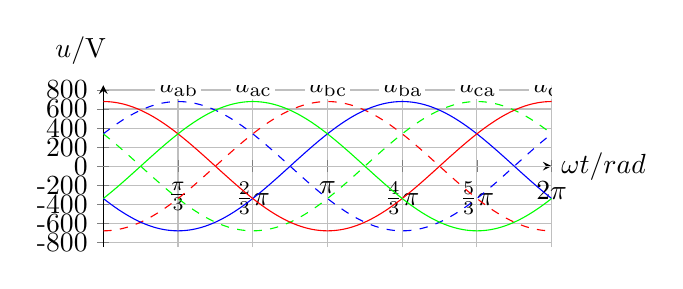
\begin{tikzpicture}
               \begin{axis}[
                   % x/y range adjustment
                   xmin=0, xmax=360,
                   ymin=-850, ymax=850,
                   samples=500,
                   axis y line=center,
                   axis x line=middle,
                   extra y ticks=0,
                   % Label text
                   xlabel={$\omega t / \text{rad}$},,
                   ylabel={$u/\mathrm{V}$},
                   % Label adjustment
                   x label style={at={(axis description cs:1,0.5)},anchor=west},
                   y label style={at={(axis description cs:-.05,.97)},anchor=south,yshift=0.2cm},
                   width=0.6\textwidth,
                   height=0.3\textwidth,
                   % x-Ticks
                   xtick={0,60,120,180,240,300,360},
                   xticklabels={,$\frac{\pi}{3}$,$\frac{2}{3}\pi$,$\pi$, $\frac{4}{3}\pi$,$\frac{5}{3}\pi$,$2\pi$},
                   xticklabel style = {anchor=north},
                   % y-Ticks
                   ytick={800,600,400,200,0,-200,-400, -600,-800},
                   yticklabels={800,600,400,200,0,-200,-400, -600,-800},
                   yticklabel style = {anchor=east},
                   % Grid layout
                   grid,
                   %grid style={line width=.1pt, draw=gray!10},
                   %major grid style={line width=.2pt,draw=gray!90},
                     ]
               % Voltage u1a(wt), u1b(wt) u1c(wt)
               \addplot[blue, domain= 0:360,dashed] {678.82*sin(x+30)};
               \addplot[red, domain= 0:360,dashed] {678.82*sin(x-90)};
               \addplot[green, domain= 0:360,dashed] {678.82*sin(x-210)};
               \addplot[blue, domain= 0:360,solid] {-678.82*sin(x+30)};
               \addplot[red, domain= 0:360,solid] {-678.82*sin(x-90)};
               \addplot[green, domain= 0:360,solid] {-678.82*sin(x-210)};
               % Label of u1c
               \node[black, fill=white, inner sep = 1pt, anchor = south] at (axis cs:180,700) {$u_{\mathrm{bc}}$}; 
               % Label of u1a
               \node[black, fill=white, inner sep = 1pt, anchor = south] at (axis cs:60,700) {$u_{\mathrm{ab}}$};           
               % Label of u1b
               \node[black, fill=white, inner sep = 1pt, anchor = south] at (axis cs:120,700) {$u_{\mathrm{ac}}$};
               % Label of u1b
               \node[black, fill=white, inner sep = 1pt, anchor = south] at (axis cs:240,700) {$u_{\mathrm{ba}}$};
               % Label of u1b
               \node[black, fill=white, inner sep = 1pt, anchor = south] at (axis cs:300,700) {$u_{\mathrm{ca}}$};
               % Label of u1b
               \node[black, fill=white, inner sep = 1pt, anchor = south] at (axis cs:360,700) {$u_{\mathrm{cb}}$};

           \end{axis}     
           \end{tikzpicture}
           \caption{Output voltage $u_\mathrm{2}(t)$ for $\alpha_\mathrm{mot}$.}
           \label{fig:Task04.2_line_voltage_B6C_with_motor_load}
   \end{figure}
\begin{solutionblock}
       



%%%%%%%%%%%%%%%%%%%%%%%%%%%%%%%%%%%%%%%%%%%%%%%%%%%%%%%%%%%%%%%%%%%%%%%%%%
\begin{solutionfigure}[htb]
    %   \documentclass{standalone}
    %   \usepackage{pgfplots}
    %   \pgfplotsset{compat=1.18} % Kompatibilität für neuere Versionen
           \centering
           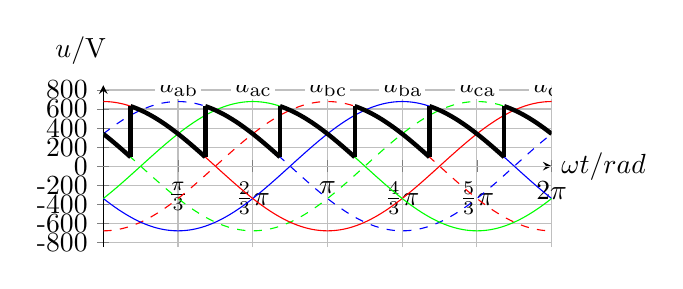
\begin{tikzpicture}
               \begin{axis}[
                   % x/y range adjustment
                   xmin=0, xmax=360,
                   ymin=-850, ymax=850,
                   samples=500,
                   axis y line=center,
                   axis x line=middle,
                   extra y ticks=0,
                   % Label text
                   xlabel={$\omega t / \text{rad}$},,
                   ylabel={$u/\mathrm{V}$},
                   % Label adjustment
                   x label style={at={(axis description cs:1,0.5)},anchor=west},
                   y label style={at={(axis description cs:-.05,.97)},anchor=south,yshift=0.2cm},
                   width=0.6\textwidth,
                   height=0.3\textwidth,
                   % x-Ticks
                   xtick={0,60,120,180,240,300,360},
                   xticklabels={,$\frac{\pi}{3}$,$\frac{2}{3}\pi$,$\pi$, $\frac{4}{3}\pi$,$\frac{5}{3}\pi$,$2\pi$},
                   xticklabel style = {anchor=north},
                   % y-Ticks
                   ytick={800,600,400,200,0,-200,-400, -600,-800},
                   yticklabels={800,600,400,200,0,-200,-400,-600,-800},
                   yticklabel style = {anchor=east},
                   % Grid layout
                   grid,
                   %grid style={line width=.1pt, draw=gray!10},
                   %major grid style={line width=.2pt,draw=gray!90},
                     ]
               % Voltage u1a(wt), u1b(wt) u1c(wt)
               \addplot[blue, domain= 0:360,dashed] {678.82*sin(x+30)};
               \addplot[red, domain= 0:360,dashed] {678.82*sin(x-90)};
               \addplot[green, domain= 0:360,dashed] {678.82*sin(x-210)};
               \addplot[blue, domain= 0:360,solid] {-678.82*sin(x+30)};
               \addplot[red, domain= 0:360,solid] {-678.82*sin(x-90)};
               \addplot[green, domain= 0:360,solid] {-678.82*sin(x-210)};

               % Voltage u2(wt)
               \addplot[black, domain= 0:21.9, solid, ultra thick] {678.82*sin(x-210)};
               \addplot[black, domain= 21.9:81.9,solid, ultra thick] {-678.82*sin(x-90)};
               \addplot[black, domain= 81.9:141.9, solid, ultra thick] {678.82*sin(x+30)}; 
                \addplot[black, domain= 141.9:201.9, solid, ultra thick] {-678.82*sin(x-210)};
                \addplot[black, domain= 201.9:261.9, solid, ultra thick] {678.82*sin(x-90)};           
               \addplot[black, domain=  261.9:321.9, solid, ultra thick] {-678.82*sin(x+30)};
               \addplot[black, domain= 321.9:360, solid, ultra thick] {678.82*sin(x-210)};
                \addplot[color=black,solid,ultra thick] coordinates{
                (21.9,95.55)
                (21.9, 629.25)
                };  
               \addplot[color=black,solid,ultra thick] coordinates{
                (81.9,95.55)
                (81.9, 629.25)
                };               
               \addplot[color=black,solid, ultra thick] coordinates{
                   (141.9,95.55)
                   (141.9, 629.25)
                };     
               \addplot[color=black,solid, ultra thick] coordinates{
                   (201.9,95.55)
                   (201.9,629.25)
                };     
               \addplot[color=black,solid, ultra thick] coordinates{
                   (261.9,95.55)
                   (261.9, 629.25)
                };
               \addplot[color=black,solid, ultra thick] coordinates{
                (321.9,95.55)
                (321.9, 629.25)
                };                    

               % Label of u1c
               \node[black, fill=white, inner sep = 1pt, anchor = south] at (axis cs:180,700) {$u_{\mathrm{bc}}$}; 
               % Label of u1a
               \node[black, fill=white, inner sep = 1pt, anchor = south] at (axis cs:60,700) {$u_{\mathrm{ab}}$};           
               % Label of u1b
               \node[black, fill=white, inner sep = 1pt, anchor = south] at (axis cs:120,700) {$u_{\mathrm{ac}}$};
               % Label of u1b
               \node[black, fill=white, inner sep = 1pt, anchor = south] at (axis cs:240,700) {$u_{\mathrm{ba}}$};
               % Label of u1b
               \node[black, fill=white, inner sep = 1pt, anchor = south] at (axis cs:300,700) {$u_{\mathrm{ca}}$};
               % Label of u1b
               \node[black, fill=white, inner sep = 1pt, anchor = south] at (axis cs:360,700) {$u_{\mathrm{cb}}$};

           \end{axis}     
           \end{tikzpicture}
           \caption{Output voltage $u_\mathrm{2}(t)$ for $\alpha = \SI{51.9}{\degree}$.}
           \label{fig:Task04_output_voltage_B6C_with_motor_load}
   \end{solutionfigure}













  

\end{solutionblock}
\subtask{List the thyristor pairs that conduct during each interval over one grid period. For each interval, specify:
    \begin{itemize}
        \item Which thyristors conduct,
        \item which input line-to-line voltage appears at the converter output.
    \end{itemize}
    Add this information to \autoref{tab:switching_intervals}, where already an example for the first interval is given.}{3}
    \subtaskGerman{Listen Sie die Thyristorpaare auf, die während jedes Intervalls in einer vollständigen Netzperiode leiten. 
    Geben Sie für jedes Teilintervall folgende Informationen an:
    \begin{itemize}
        \item Welche Thyristoren leiten,
        \item die am Ausgang des Konverters durchgeschaltete Leiter-Leiter-Spannung von dessen Eingang.
    \end{itemize}
    Fügen Sie dies in \autoref{tab:switching_intervals} ein, wo bereits ein Beispiel für das erste Intervall gegeben ist.}
    \begin{table}[ht]
    \centering  
    \begin{tabular}{|c|c|c|}
        \hline
        \textbf{Interval (° electrical)} & \textbf{Conducting Thyristor Pair} & \textbf{Load Voltage $u_\mathrm{2}(t)$} \\
        \hline
                    $30+\alpha$          &    $T_\mathrm{1}, T_\mathrm{4}$      &     $u_\mathrm{ab}$        \\
        \hline
               &                                      &                                      \\
        \hline
               &                                      &                                      \\
        \hline
               &                                      &                                      \\
        \hline
               &                                      &                                      \\
        \hline
               &                                      &                                      \\
        \hline
    \end{tabular}
    \caption{Switching intervals, conducting thyristor pairs, and corresponding load voltage.}
    \label{tab:switching_intervals}
\end{table}
\begin{solutionblock}
       \begin{table}[ht]
    \centering  
    \begin{tabular}{| >{\color{blue}}c | >{\color{blue}}c | >{\color{blue}}c |}
        \hline
        \textbf{\textcolor{black}{Interval (° electrical)}} & \textbf{\textcolor{black}{Conducting Thyristor Pair}} & \textbf{\textcolor{black}{Load Voltage $u_\mathrm{2}(t)$}} \\
        \hline
                    $30+\alpha$          &    $T_\mathrm{1}, T_\mathrm{4}$      &     $u_\mathrm{ab}$         \\
        \hline
                    $90+\alpha$          &    $T_\mathrm{1}, T_\mathrm{6}$      &     $u_\mathrm{ac}$         \\
        \hline
                    $150+\alpha$         &    $T_\mathrm{3}, T_\mathrm{6}$      &     $u_\mathrm{bc}$         \\
        \hline
                    $210+\alpha$         &    $T_\mathrm{3}, T_\mathrm{2}$      &     $u_\mathrm{ba}$         \\
        \hline
                    $270+\alpha$         &    $T_\mathrm{5}, T_\mathrm{2}$      &     $u_\mathrm{ca}$         \\
        \hline
                    $330+\alpha$         &    $T_\mathrm{5}, T_\mathrm{4}$      &     $u_\mathrm{cb}$         \\
        \hline
    \end{tabular}
    \caption{Switching intervals, conducting thyristor pairs, and corresponding load voltage.}
    \label{stab:switching_intervals}
\end{table}
\end{solutionblock}
\subtask{Given the fundamental input current amplitude $\hat{i}^\mathrm{(1)}_\mathrm{1a}=\SI{55.13}{\ampere}$ and
nominal motor current $I_\mathrm{mot}$, calculate the average active power supplied to the motor and the 
fundamental reactive power absorbed from the grid.}{3}
\subtaskGerman{Basierend auf der Grundwellenamplitude des Eingangsstroms $\hat{i}^\mathrm{(1)}_\mathrm{1a}=\SI{55.13}{\ampere}$ und des Nennstroms $I_\mathrm{mot}$ des Motors,
berechnen Sie die durchschnittliche Wirkleistung, die dem Motor zugeführt wird und die Grundwellenblindleistung, die dem Netz entnommen.}
\begin{solutionblock}
   
    $$ P_\mathrm{mot} = U_\mathrm{mot,term} I_\mathrm{mot}=\SI{400}{\volt} \cdot \SI{50}{\ampere} = \SI{20}{k\watt}.$$

    The input voltage $U_\mathrm{1}^\mathrm{(1)}$ corresponds to $U_\mathrm{1}$, so that the apparent power results to

        $$    S_\mathrm{mot}^\mathrm{(1)} = 3 U_\mathrm{1} \frac{\hat{i}_\mathrm{1a}^\mathrm{(1)}}{\sqrt{2}}= 3 \cdot \SI{277}{\volt} \cdot \frac{\SI{55.13}{\ampere}}{\sqrt{2}}= \SI{32.40}{k\volt\ampere}.$$
    The reactive power is calculated by

        $$    Q_\mathrm{mot}^\mathrm{(1)} = 3 U_\mathrm{1} \frac{\hat{i}_\mathrm{1a}^\mathrm{(1)}}{\sqrt{2}} \sin{(\alpha_\mathrm{mot})}
            = 3 \cdot \SI{277}{\volt} \cdot \frac{\SI{55.13}{\ampere}}{\sqrt{2}}\sin{(51.9)}= \SI{25.49}{k\volt\ampere}.$$

\end{solutionblock}
\subtask{Using the same value for $\hat{i}^\mathrm{(1)}_\mathrm{1a}$ as in the previous subtask, calculate the THD of the phase current $i_\mathrm{1a}(\omega t)$.}{2}
\begin{hintblock}
    use the same THD formula given in the previous task.
\end{hintblock}
\subtaskGerman{Berechnen Sie den THD des Phasenstroms $i_\mathrm{1a}(\omega t)$ unter der Annahme, dass der Grundwellenstrom
am Konvertereingang dem Wert der vorherigen Teilaufgabe entspricht.}
\begin{germanhintblock}
    verwenden Sie dieselbe THD-Formel wie in der vorherigen Aufgabe.
\end{germanhintblock}
\begin{solutionblock}
    The effective value of the fundamental current component is
    
    $$    I^\mathrm{(1)}_\mathrm{1a} = \frac{\hat{i}^\mathrm{(1)}_\mathrm{1a}}{\sqrt{2}} = \SI{38.98}{\ampere},$$
    while the effective value of the input phase current $i_\mathrm{1a}$ is 

    $$    I_\mathrm{1a} = \sqrt{\frac{2}{2\pi}\left(\int_{0}^{\frac{\pi}{3}} I^2_\mathrm{2}\mathrm{d}\omega t + \int_{\frac{2\pi}{3}}^{\pi} I^2_\mathrm{2}\mathrm{d}\omega t\right)} =  \frac{I_\mathrm{2}\cdot \sqrt{2}}{\sqrt{3}} \approx \SI{40.82}{\ampere}.$$
    So, the THD is

    $$    \mathrm{THD} = \sqrt{\left(\frac{I^2_\mathrm{1a}}{(I^\mathrm{(1)}_\mathrm{1a})^2}\right)-1} = \SI{31.086}{\percent}.$$  
\end{solutionblock}
\subtask{State the effect of changing the number of pulses $p$ (by using other converter topologies) on the maximum achievable voltage and THD of the input current.}{2}
\subtaskGerman{Geben Sie den Einfluss einer veränderten Pulszahl $p$ (durch Nutzung anderer Konvertertopologien) auf die maximal erreichbare Spannung und den THD des Eingangsstroms an.}
\begin{solutionblock}
    Increasing the number of pulses $p$:
    \begin{itemize}
        \item Increases the maximum achievable DC output voltage.
        \item Reduces the THD of the input current.
    \end{itemize}
\end{solutionblock}






